\documentclass[12pt, openany]{report}
\usepackage[utf8]{inputenc}
\usepackage[T1]{fontenc}
\usepackage[a4paper,left=2cm,right=2cm,top=2cm,bottom=2cm]{geometry}
\usepackage[frenchb]{babel}
\usepackage{libertine}
\usepackage[pdftex]{graphicx}

\setlength{\parindent}{0cm}
\setlength{\parskip}{1ex plus 0.5ex minus 0.2ex}
\newcommand{\hsp}{\hspace{20pt}}
\newcommand{\HRule}{\rule{\linewidth}{0.5mm}}

\usepackage{subfig}
\usepackage{float}

\usepackage{amsmath}
\usepackage{amssymb}
\usepackage{latexsym}
\usepackage{algorithm,algorithmic}

%% TIKZ
\usepackage{tikz}
\usetikzlibrary{trees,%
                shapes,%
                plotmarks,%
                arrows,%
                er,%
                automata,%
                petri,%
                topaths}%
\usepackage{tkz-graph}
\usepackage{lineno, setspace}
%% TIKZ


%\setlength{\textheight}{22cm}
%\setlength{\textwidth}{17.3cm}
%\setlength{\topmargin}{-0.5cm}
%\setlength{\oddsidemargin}{-0.5cm}

\newtheorem{lemma}{Lemme}
\newtheorem{definition}{Définition}
\newtheorem{theorem}{Théorème}
\newtheorem{proposition}{Proposition}
\newtheorem{conjecture}{Conjecture}
\newtheorem{corollary}{Corollaire}
\newtheorem{remark}{Remarque}

\newcommand{\bpr}{{\bf {Preuve }}}
\newcommand{\epr}{\hfill$\Box$\\}
\newcommand{\eprs}{\hfill$\Box$}

% Commandes pour algorithm
%\newcommand{\algorithmicrequire}{\textbf{Require:}} 
%\newcommand{\algorithmicensure}{\textbf{Ensure:}} 
\renewcommand{\algorithmicend}{\textbf{fin}} 
\renewcommand{\algorithmicif}{\textbf{si}} 
\renewcommand{\algorithmicthen}{\textbf{alors}} 
\renewcommand{\algorithmicelse}{\textbf{sinon}} 
%\newcommand{\algorithmicelsif}{\algorithmicelse\ \algorithmicif} 
%\newcommand{\algorithmicendif}{\algorithmicend\ \algorithmicif} 
\renewcommand{\algorithmicfor}{\textbf{pour}} 
\renewcommand{\algorithmicforall}{\textbf{pour tout}} 
\renewcommand{\algorithmicdo}{\textbf{faire}}
%\newcommand{\algorithmicendfor}{\algorithmicend\ \algorithmicfor} 
\renewcommand{\algorithmicwhile}{\textbf{tant que}} 
%\newcommand{\algorithmicendwhile}{\algorithmicend\ \algorithmicwhile} 
\renewcommand{\algorithmicloop}{\textbf{boucle}} 
%\newcommand{\algorithmicendloop}{\algorithmicend\ \algorithmicloop} 
\renewcommand{\algorithmicrepeat}{\textbf{répéter}} 
\renewcommand{\algorithmicuntil}{\textbf{jusqu'à}} 
\renewcommand{\algorithmicprint}{\textbf{afficher}} 
\renewcommand{\algorithmicreturn}{\textbf{retourner}}




\begin{document}

\begin{titlepage}
  \begin{sffamily}
  \begin{center}

    % Upper part of the page. The '~' is needed because \\
    % only works if a paragraph has started.
%    \includegraphics[scale=0.04]{../Images/im1.png}~\\[1.5cm]

    \textsc{\LARGE Travaux Personnels Encadrés 1\degre S}\\[2cm]

    \textsc{\Large Thème : avancées scientifiques et réalisations techniques}\\[1.5cm]

    % Title
    \HRule \\[0.4cm]
    { \huge \bfseries La bio-informatique\\[0.4cm] }

    \HRule \\[2cm]
    \includegraphics[scale=1]{Images/im1.png}
    \\[2cm]

    % Author and supervisor
    \begin{minipage}{0.4\textwidth}
      \begin{flushleft} \large
        A. A.\\
L. B.\\
J. D.\\
      \end{flushleft}
    \end{minipage}
    \begin{minipage}{0.4\textwidth}
      \begin{flushright} \large
Première S\\
      \end{flushright}
    \end{minipage}

    \vfill

    % Bottom of the page
    {\large 2014-2015}

  \end{center}
  \end{sffamily}
\end{titlepage}

\tableofcontents


%\abstract{Ces notes présentent la théorie des graphes, les algorithmes et les structures de données nécessaires à une utilisation de ce modèle par ordinateur.}

\chapter{Introduction}

La bio-informatique est un domaine de recherche qui analyse et interprète des données biologiques, au moyen de méthodes informatiques, afin de créer de nouvelles connaissances en biologie. Elle contribue aussi à la guérison du cancer, qui est une pathologie caractérisée par la présence d'une ou plusieurs tumeur(s) maligne formée à partir de la transformation par mutations ou instabilité génétique d'une cellule initialement normal. 

A travers ce sujet, nous allons essayer de répondre à la question suivante : La bio-informatique permet-elle vraiment d'aider au traitement des cancers ? Dans un premier temps, nous verrons comment intervient la médecine personnalisée pour le cancer, puis dans un second temps nous verrons les limites de la bio-informatique. Pour finir nous illustrerons notre TPE grâce à l’étude du projet SHIVA et du projet WINTHER. 



\chapter{La médecine personnalisée pour le cancer}

Le but principal de la bio-informatique est de trouver un traitement au patient grâce à la médecine personnalisée. La médecine personnalisée consiste, en cancérologie, à rechercher le traitement le mieux adapté au patient en fonction des caractéristiques génétiques de sa tumeur et de l'environnement du patient. On prélève des cellules cancéreuses métastatiques (en général par biopsie, mais des techniques sont développées pour récupérer celles qui circulent dans le sang) ; 
on analyse le génome de ces cellules, et l'on y recherche des anomalies ; 
on compare ensuite ces résultats avec des banques de données (mutations trouvées chez d'autre patients, médicaments...) afin de déterminer le traitement correspondant le mieux au profil génétique de la tumeur.

\section{Les outils de la médecine personnalisée}

\subsection{Séquençage}

Le  séquençage\footnote{voir lexique page~\pageref{lexique}} est une technique qui a révolutionnée la biologie moléculaire dans les années 1970, soit seulement une vingtaine d’années après l’établissement de la structure de l’ADN  par Watson et Crick. 

\begin{figure}[h]
\begin{center}
    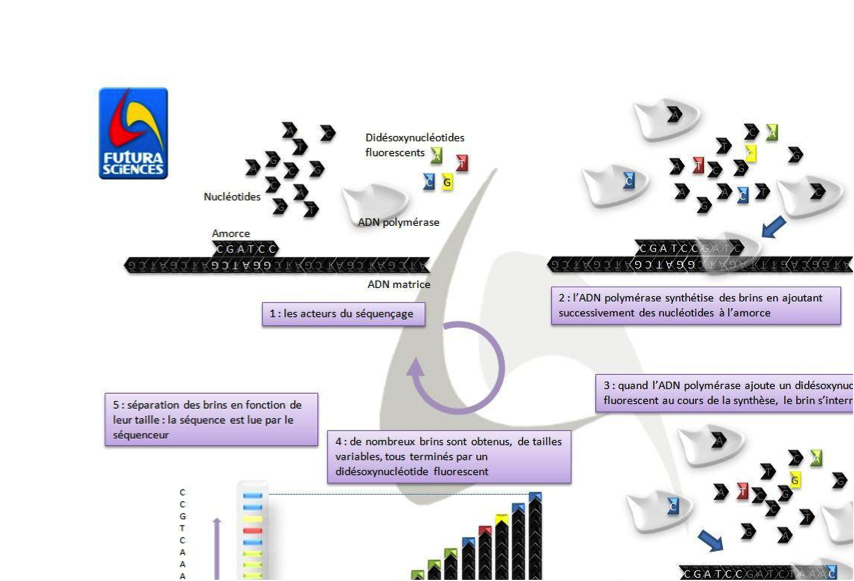
\includegraphics[scale=1]{Images/im2.png}
\caption{Les différentes étapes du séquençage}\label{fig:séquençage}
\end{center}
\end{figure}

L’ADN\footnote{voir lexique page~\pageref{lexique}}, contenu dans chacune de nos cellules, contient l’information nécessaire à l’expression des gènes, une information importante aux yeux des biologistes.
La connaissance de sa séquence, c'est-à-dire la succession des bases de l’ADN (adénine, cytosine, guanine, thymine), est aujourd’hui de plus en plus facile à déterminer.

Le séquençage se déroule initialement dans un tube à essai dans lequel il y a de l'ADN à séquencer, des nucléotides, une amorce et de l'ADN polymérase. Tous ces acteurs sont en très grande quantité, donc la réaction du séquençage fait intervenir de multiples réactions. 

Tout d'abord l’ADN polymérase utilise aléatoirement les nucléotides présents dans le milieu pour copier le brin matrice en synthétisant un ADN de séquence complémentaire, du moment que la base (A, C, G ou T) est respectée. Lorsque l’ADN polymérase choisit par hasard un didésoxynucléotide (ce qui est rare puisqu'il y en a moins que des nucléotides) et qu’elle l’incorpore dans la chaîne en synthèse, celle-ci s’interrompt prématurément. Puisque chaque didésoxynucléotide est marqué par un fluorochrome différent (A vert, T rouge, G jaune et C bleu), une chaîne qui se termine par exemple par un A sera verte. Puisqu'il y a eu un très grand nombre de réactions de synthèse dans le tube, il existe statistiquement des chaînes de toutes les tailles (correspondant à un arrêt de la synthèse à chaque nucléotide) et beaucoup de fragments de même taille. Toutes les chaînes commencent au même endroit sur l'ADN matrice, donc toutes celles qui ont la même longueur se terminent par le même didésoxynucléotude marqué. Il est alors possible de séparer les chaînes d’ADN obtenues en fonction de leur taille, sur un gel d’acrylamide en présence d'un courant électrique. Plus les chaînes sont courtes, plus elles migrent loin et tous les fragments d'une même taille migrent à la même distance. On obtient alors une succession de bandes colorées, chacune correspondant au dernier nucléotide incorporé. Il suffit alors de lire la succession des couleurs pour connaître l’ordre des nucléotides, c'est-à-dire la séquence de l’ADN, étape assurée automatiquement par les détecteurs du séquenceur.

\begin{figure}[H]
\begin{center}
    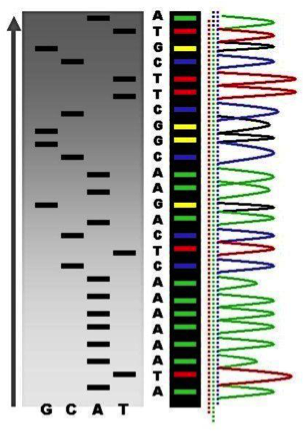
\includegraphics[scale=0.9]{Images/im3.png}
\caption{La séquence peut se lire à l'œil sur un gel d'acrylamide grâce aux bandes radioactives visibles dans chaque poche (à gauche, en noir et blanc), ou au séquenceur capable de détecter les intensités de fluorescence de chaque bande (à droite, en couleurs).}
\end{center}
\end{figure}

%Illustration 2: La séquence peut se lire à l'œil sur un gel d'acrylamide grâce aux bandes radioactives visibles dans chaque poche (à gauche, en noir et blanc), ou au séquenceur capable de détecter les intensités de fluorescence de chaque bande (à droite, en couleurs).

\subsection{Algorithmes}

Après avoir trouver les séquences de nucléotides du patient atteint de cancer, il faut les comparer avec d’autres. Pour cela, on utilise l’alignement de séquences. Celui-ci permet de trouver des similarités entre les séquences analysées. Ces similarités sont dues à une origine évolutive commune (homologie) ou à des fonctions semblables.
D'autre part, l'alignement de séquences permet de vérifier l'absence de similarité entre séquences afin de vérifier l'unicité d'hybridation (croisement)  d'une séquence donnée et donc sa spécificité.

Donc l'alignement de séquences a pour buts :
\begin{enumerate}
\item	Identifier au sein d'une banque une séquence obtenue en laboratoire de biologie.											
 \item Localiser une séquence d'acide nucléique\footnote{voir lexique page~\pageref{lexique}} au sein du génome d'un organisme.              											
\item Identifier un rôle à une molécule séquencée par comparaison avec des molécules de fonctions similaires déjà répertoriées.							
\item Réaliser une étude phylogénétique.									
\item Prédire la structure secondaire (tertiaire) d'une protéine.
\end{enumerate}

Pour comparer des séquences il faut alors utiliser des alorithmes. BLAST (Basic Local Alignment Search Tool) est un outil développé par Genbank qui permet de d'aligner des séquences contre l'ensemble des séquences de la banque. Nous allons comprendre comment il fonctionne.

\begin{figure}[H]
\begin{center}
    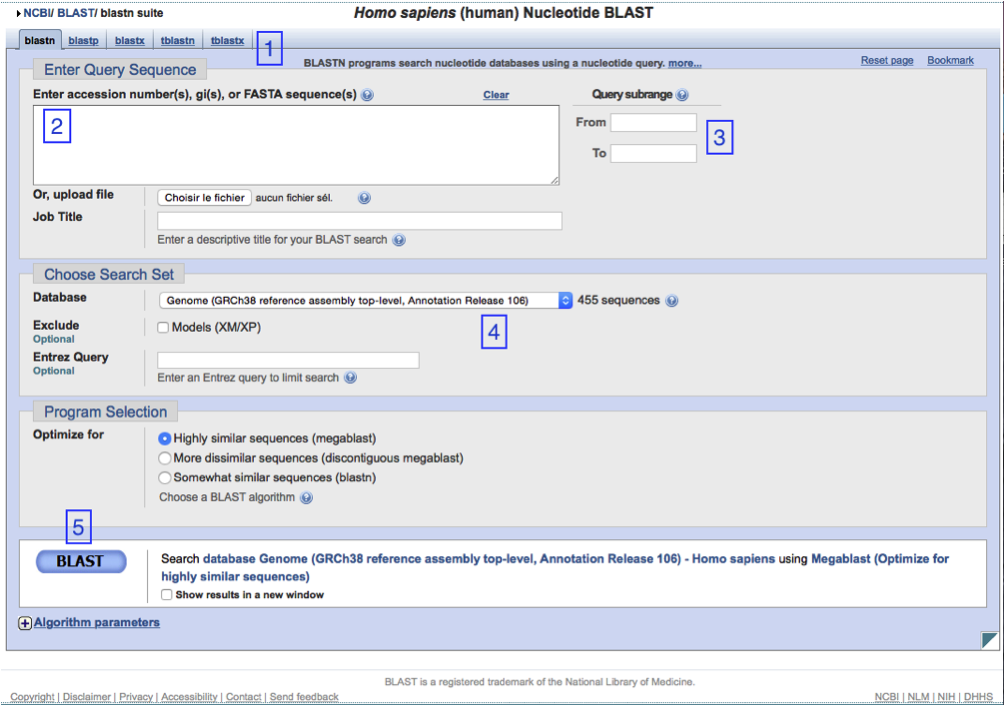
\includegraphics[scale=0.9]{Images/im4.png}
\caption{Page d’acceuil de BLAST}
\end{center}
\end{figure}

Pour commencer, il faut choisir une version de BLAST suivant nos séquences (1). 

Blastn aligne entre des séquences de nucléotides, Blastp aligne entre des séquences de protéines, Blastx aligne une séquence de nucléotides “traduite” contre des nucléotides “traduites" de la banque… 

Ensuite, il faut rentrer la séquence à étudier (2) et on peut éventuellement délimiter la zone à aligner (3). Puis on choisit la base de comparaison qui est dans la banque de donnée (4). Pour finir, on lance l’algorithme d’alignement (5). 
 
	Puis BLAST nous donne 4 types de résulats:
\begin{enumerate}
\item un récapitulatif (Figure~\ref{fig:reca});
\item une représentation graphique des résultats (Figure~\ref{fig:graphe}) :
\begin{itemize}
\item les traits de couleur correspondent à un alignement entre la séquence soumise et une séquence de la banque ;
\item la couleur correspond au score ;
\item la longueur correspond à la taille de l'alignement ;
\end{itemize}

\item une représentation globale des résultats (Figure~\ref{fig:global}).

Chaque ligne correspond à un trait coloré de la représentation graphique.

On trouve dans ce tableau le score et l'E-value: le score permet de comparer deux alignements et dire lequel est a priori le plus performant. L’E-value est une aide à la décision et ne s'interprète pas seule pour décider si l'alignement est biologiquement significatif. A la différence du score, l' E-value prend en compte la taille de la banque ;

\item une description des résultats des alignements (Figure~\ref{fig:align}):
\begin{itemize}
\item Query : la séquence soumise,
\item Subject : la séquence de la base de données.
\end{itemize}
\end{enumerate}

\begin{figure}[H]
\begin{center}
    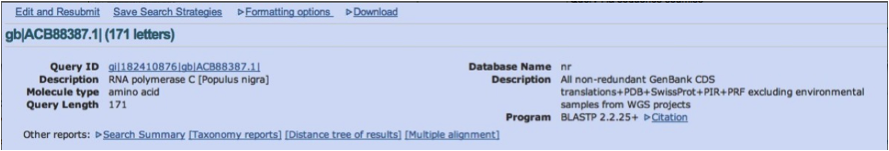
\includegraphics[scale=1]{Images/im5.png}
\caption{BLAST : récapitulatif}\label{fig:reca}
\end{center}
\end{figure}

\begin{figure}[H]
\begin{center}
    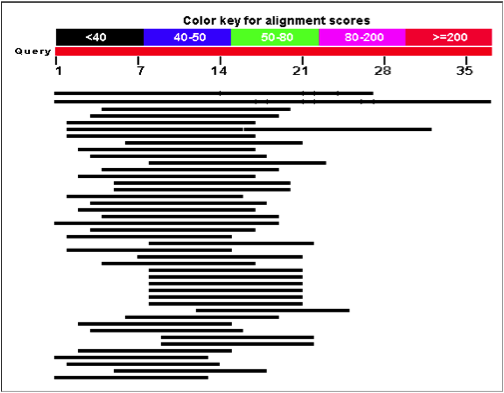
\includegraphics[scale=1]{Images/im6.png}
\caption{BLAST : représentation graphique des résultats}\label{fig:graphe}
\end{center}
\end{figure}

\begin{figure}[H]
\begin{center}
    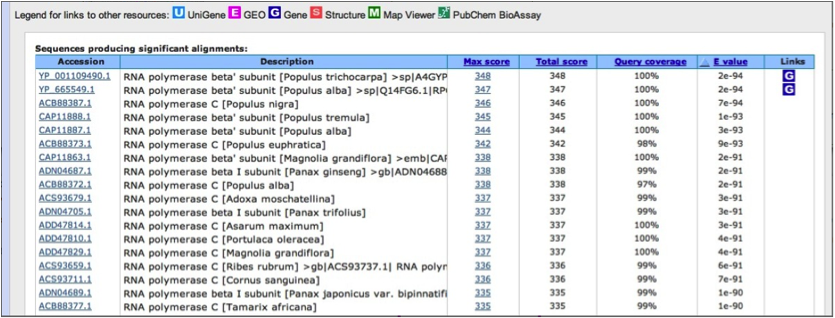
\includegraphics[scale=1]{Images/im7.png}
\caption{BLAST : représentation globale des résultats}\label{fig:global}
\end{center}
\end{figure}

\begin{figure}[H]
\begin{center}
    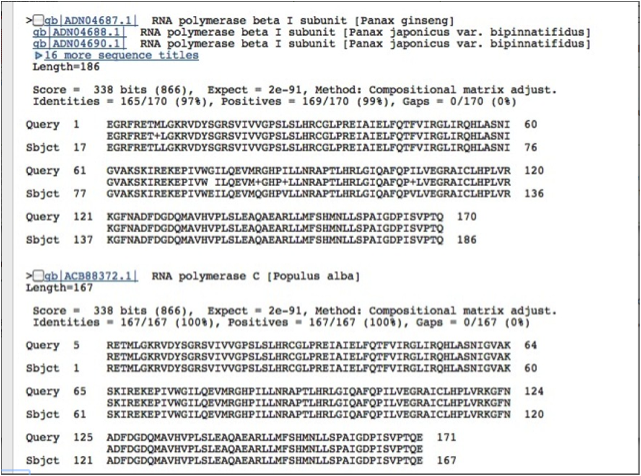
\includegraphics[scale=1]{Images/im8.png}
\caption{BLAST : description des résultats des alignements}\label{fig:align}
\end{center}
\end{figure}

Grâce à tout ces résultats, les chercheurs analysent et essaient de trouver un traitement qui conviendra au patient suivant ses gènes.

\section{Les utilisations de la médecine personnalisée}

\subsection{Des prédispositions génétiques}

	Si cette personnalisation de la médecine en fonction du patrimoine génétique est possible actuellement, c’est grâce aux progrès technologiques qui ont permis de réduire les coûts et les temps d’analyse du séquençage  et du génotypage\footnote{voir lexique page~\pageref{lexique}} de l’ADN. 

De nos jours, il est possible de séquencer plusieurs centaines de gènes en quelques semaines et pour un prix relativement raisonnable, qui continue de baisser. Des sociétés privées proposent même pour quelques centaines d’euros le génotypage de l’ADN personnel, accompagné d’un rapport sur les risques potentiels de développer une maladie. La liste est longue et non exhaustive : asthme, diabète, Alzheimer, Parkinson, arthrose, hypertension, maladies cardiovasculaires, certains cancers, autisme, schizophrénie, troubles bipolaires\ldots

\begin{figure}[H]
\begin{center}
    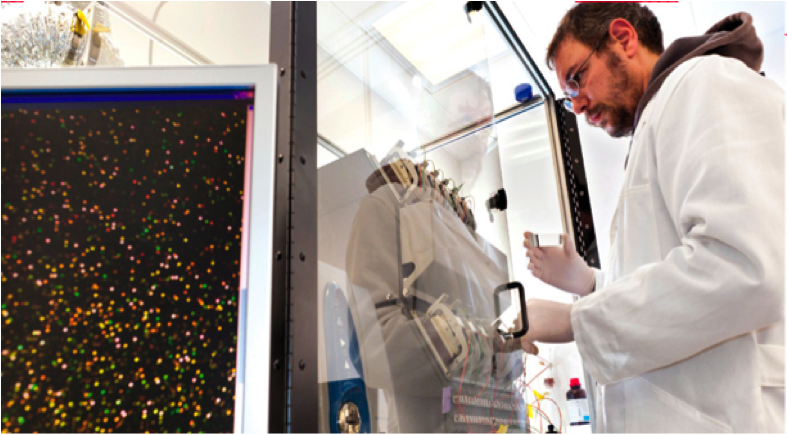
\includegraphics[scale=1]{Images/im10.png}
\caption{Séquençage à haut débit}
\end{center}
\end{figure}

\begin{figure}[H]
\begin{center}
    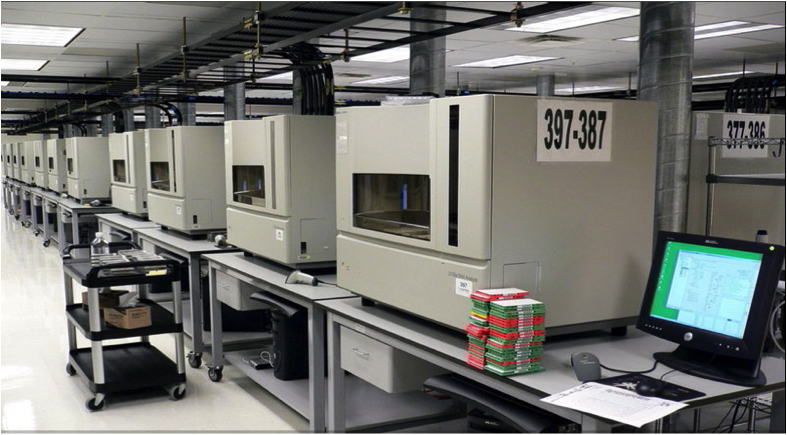
\includegraphics[scale=1]{Images/im11.png}
\caption{Séquenceur d’ADN}
\end{center}
\end{figure}
	
Au début la médecine personnalisé consistait à caractériser les prédispositions génétiques à certaines maladies. Ces informations peuvent permettre d’adapter la surveillance pour les personnes à risque. 
	
	Selon l’Institut national contre le cancer (INCa), environ deux femmes sur mille présentent un risque de 45 à 65\% plus élevé que la population générale de développer un cancer du sein. Quant au cancer de l’ovaire, ce risque est pour ces femmes de 11 à 39\% plus élevé à cause de  deux gènes dénommés BRCA1 et BRCA2 qui ne participent plus correctement à certains mécanismes de réparation de l’ADN lorsqu'ils sont mutés. Des cellules saines peuvent alors devenir cancéreuses.

\subsection{Des traitements ciblés}

Actuellement, la cible première de la médecine personnalisée est le cancer. 

En effet, l’étude des altérations génétiques présentes dans le génome des tumeurs permet de personnaliser le diagnostic et le pronostic. Ces mutations jouent un rôle important dans le développement d’un cancer. 

Dans la pratique clinique, elles peuvent alors servir de biomarqueurs. Ces derniers signalent la présence d’une maladie ou la réponse des traitements grâce à une caractéristique mesurable. 

La glycémie, par exemple, est un biomarqueur qui permet de caractériser le diabète ainsi que l’efficacité des molécules antidiabétiques. 

Dans le cas du cancer, l’absence ou la présence de ces mutations génétiques dans une biopsie peut indiquer si la tumeur est bénigne ou maligne, et détermine son agressivité. Par exemple, environ 15\% des cancers du sein résistent aux traitements classiques et ont tendance à former des métastases. Ces tumeurs présentent généralement la même mutation : une surexpression du gène HER2. 

« Mieux comprendre les altérations du génome tumoral permet d’améliorer le diagnostic et le pronostic mais aussi de proposer un traitement personnalisé », explique Jessica Zucman-Rossi\cite{ZR2013}. Car elles peuvent être utilisées comme des cibles thérapeutiques. On peut citer l’un des premiers succès de la génomique dans le traitement du cancer grâce au trastuzumab. Ce médicament, autorisé sur le marché en France en 2000, cible directement les récepteurs HER2 des cellules cancéreuses et épargne ainsi les tissus sains. On y gagne une thérapie plus efficace et moins d’effets secondaires.

\begin{figure}[H]
\begin{center}
    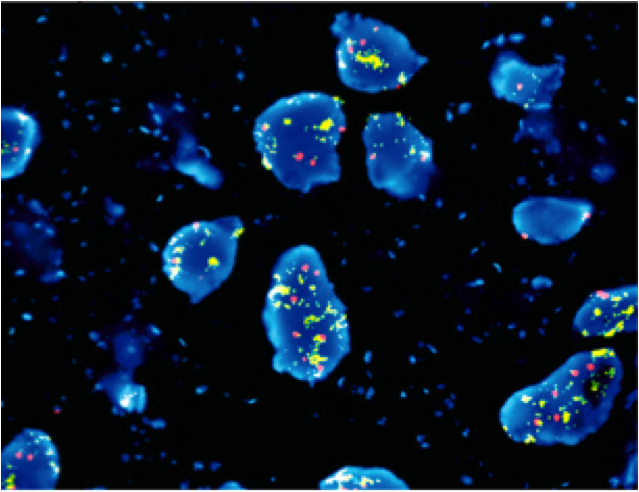
\includegraphics[scale=1]{Images/im12.png}
\caption{L'amplification anormale du nombre de copies du gène MDM2 (vert) dans le noyau (bleu) de cellule tumorale est le signe d'un cancer des cellules graisseuses (liposarcome).}
\end{center}
\end{figure}

\chapter{Les limites de la médecine personnalisée}

\section{L'hétérogénéité intratumorale}

\subsection{Qu’est-ce que l’hétérogénéité intratumorale ?}

Depuis des années on sait que le cancer commence à se développer lorsque le génome d’une cellule subit des anomalies oncogénétiques\footnote{voir lexique page~\pageref{lexique}}, c’est à dire lui donnant la capacité de se multiplier indéfiniment. Les tumeurs ne constituent pas un ensemble de clones de cette unique cellule anormale d’origine, mais plutôt une mosaïque de clones issus de plusieurs cellules anormales. 

On est donc face à un système complexe très hétérogène. C’est ce que l’on appelle l’hétérogénéité intratumorale.

 \begin{figure}[H]
\begin{center}
    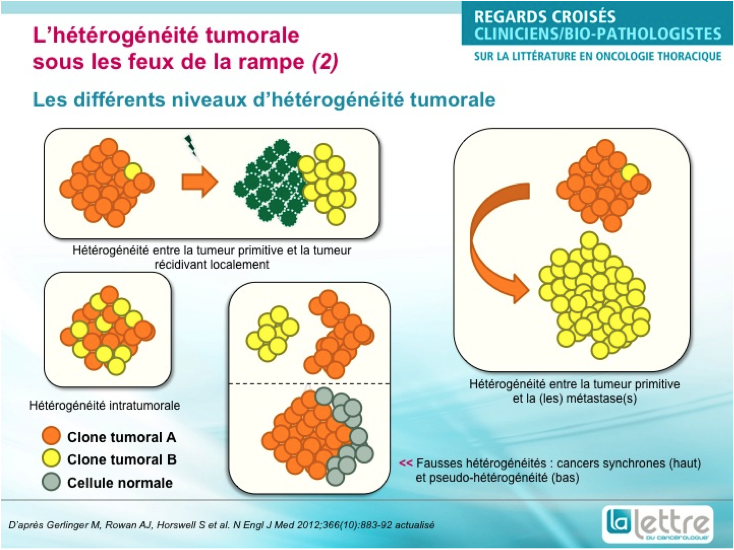
\includegraphics[scale=1]{Images/im13.png}
\caption{L’hétérogénéité intratumorale}
\end{center}
\end{figure}

\subsection{En quoi est-ce un problème dans le traitement du cancer grâce à la médecine personnalisée ?}

Lors d’un traitement grâce à la médecine personnalisée, le traitement est prescrit en fonction des caractéristiques moléculaires de la tumeur. Mais le plus souvent, ce choix se base sur la recherche de caractéristique(s) particulière(s) sur une seule biopsie. 

Lorsqu’on procède à celle-ci, on ne détecterait finalement que 50\% des anomalies génétiques propres au cancer du patient. Avec une tumeur hétérogène, le risque est donc de proposer une thérapie ciblée efficace uniquement sur une sous-population de cellules cancéreuses (celles qu’on a prélevées). Plus l'hétérogénéité est grande, plus la réponse à un traitement est donc aléatoire. 

\subsection{Existe-il des solutions face à cette obstacle ?}

Tous les patients ne sont pas à la même enseigne : certains présentent une forte hétérogénéité intratumorale, tandis que chez d'autres, elle est très peu marquée. 

Il est donc nécéssaire de quantifier cette hétérogénéité, afin de mieux orienter les patients : la médecine personnalisée ayant peu de chances d'être efficace chez des personnes identifiées comme ayant une forte hétérogénéité intratumorale, ces personnes pourraient être orientées vers d'autres stratégies. 

Des outils se mettent en place pour quantifier l'hétérogénéité d'une tumeur mais les solutions n’ont pas encore abouti. 

En effet, les cellules tumorales circulent dans le sang pour coloniser d’autres organes et un processus naturel de dégradation des cellules (normales et cancéreuses) fait qu’une partie de leur matériel génétique se retrouve dans le sang. En récupérant ces informations génétiques grâce à une simple prise de sang, on pourrait avoir une vision globale des mutations génétiques du cancer du patient. Non seulement cela donnerait un aperçu plus global que celui que pourrait nous offrir de multiples biopsies, mais cette opération pourrait également être répétée sans risque pour le patient. 

Une fois ces mutations identifiées, une analyse bio-informatique permettrait d’établir l’arbre phylogénétique de ces mutations. Plus simplement, d’identifier les mutations successives qui, au cours de l’évolution du cancer, lui ont conféré un avantage significatif (en terme de croissance ou de résistance au traitement) afin qu’elles deviennent les cibles prioritaires des traitements. 

Dans la Figure~\ref{fig:visu}, on peut observer les différentes mutations représentées par les lignes rouges dans les première cellules cancéreuses (ligne jaune) puis dans les metastases\footnote{voir lexique page~\pageref{lexique}} (ligne verte).

  \begin{figure}[H]
\begin{center}
    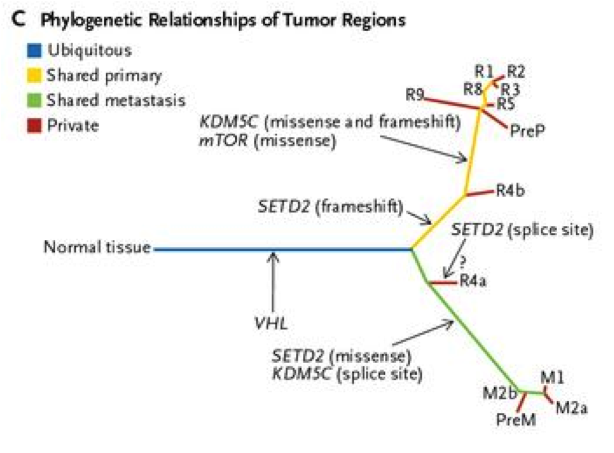
\includegraphics[scale=0.6]{Images/im14.png}
\caption{Exemple de visualisation des différentes mutations constatées chez un patient atteint de cancer du rein au stade avancé - New England Journal of Medicine, vol. 366, pp. 883-892, 2012.}\label{fig:visu}
\end{center}
\end{figure}

Une autre solution est aussi envisagée. Il s’agit de comprendre les mécanismes qui créent ces hétérogénéités afin que les thérapies personnalisées fonctionnent. 

Nous savons à présent qu'il faut chercher le mécanisme qui crée l'hétérogénéité, c'est a dire très probablement du coté de la machine moléculaire qui répare l'ADN : quelles molécules de cette machinerie sont impliquées dans l'apparition de nouvelles mutations ? 

Une fois identifiées, ces molécules constitueront de nouvelles cibles pour des médicaments.
 Comprendre les mécanismes permettrait de combiner ces thérapies avec d'autres évitant l'adaptation de la tumeur.

\section{Les limites éthiques, juridiques et socio-économiques}
 
\subsection{Problèmes éthiques et juridiques}

\subsubsection{Quels problèmes éthiques et juridiques la médecine personnalisée entraîne-t-elle ?} 

Le traitement par la médecine personnalisée pose des problèmes éthiques et judiciaires sur la confidentialité et le respect de la vie privée, suite aux nombreuses informations génétiques résultant du séquençage du génome des patients, notamment concernant des prédispositions. 

En effet, l’ensemble des données n’est pas nécessaire pour la prise en charge du malade. Et le surplus pourrait être très utile à la recherche. Une fois qu'un médecin aura en main les renseignements sur le patrimoine génétique d'un individu, comment gérera-t-il cette information ? Sera-t-il tenu d'informer le patient et même la famille s'il sait que l'individu, et peut-être d'autres membres de sa famille, présentent des risques de développer telle ou telle maladie ? De plus, l'utilisation de données génétiques dans le domaine médical peut également mener à de la discrimination génétique par les assurances ou les employeurs.
 
 \begin{figure}[H]
\begin{center}
    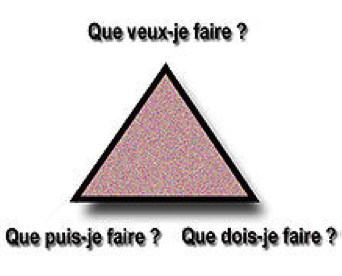
\includegraphics[scale=1]{Images/im15.png}
\end{center}
\end{figure}

\subsubsection{Quelles solutions peuvent-être envisagé face a ce problème ?}

L'établissement de normes juridiques précises semble plus que nécessaire dans ce domaine. D’après le rapport de MM. Alain CLAEYS et Jean-Sébastien VIALATTE, fait au nom de l'Office parlementaire d'évaluation des choix scientifiques et technologiques 
n\degre 306 (2013-2014) - 22 janvier 2014 : "Ils préconisent une réforme de la formation des études de santé. Ils insistent sur la préservation de l'égal accès de tous les citoyens aux nouvelles thérapies ciblées et sur le maintien du système solidaire de santé publique. Ils recommandent de mieux informer les citoyens et de faciliter l'intervention des associations de malades à tous les niveaux du parcours de santé."
 
Il faut aussi plus impliquer le patient, lui demander quels types d’informations il souhaite avoir, et lui fournir les éléments qui lui permettent de comprendre ces résultats. Étant donnée que le surplus de données pourrait être très utile à la recherche, il faudrait alors demander systématiquement l’autorisation du patient pour l’utilisation de telles données en recherche, sans pour autant que que ce soit pour un projet précis.
 
Claire Julian-Reynier, médecin responsable de l’équipe "Cancer, biomédecine et société" (CAN-BIOS), à l’Institut Paoli-Calmettes à Marseille explique : “En menant une enquête auprès de personnes  atteintes d’un cancer du sein, nous avons constaté qu’elles étaient très favorables à leur utilisation étant donné le bénéfice en termes de traitement, mais, par ailleurs, un certain nombre de malentendus et d’inquiétudes ont été constatés sur les résultats obtenus. Passer plus de temps pour expliquer et discuter doit leur permettre de prendre une part plus active et plus éclairée aux décisions concernant leur traitement. Avec pour conséquences de mieux supporter la période d’annonce des traitements et leur vécu ultérieur."
 
 \begin{figure}[H]
\begin{center}
    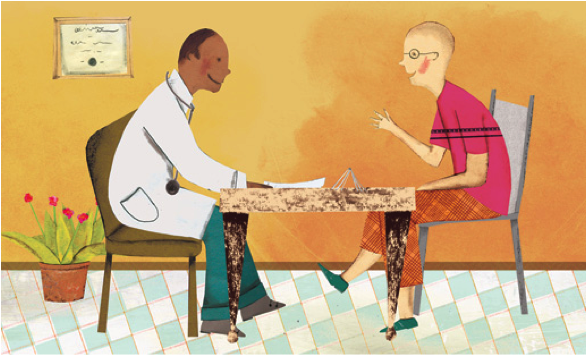
\includegraphics[scale=1]{Images/im16.png}
\end{center}
\end{figure}

\subsection{Problèmes socio-économiques}

\subsubsection{Quels problèmes socio-économiques la médecine personnalisée entraîne-t-elle ?} 

La médecine personnalisée pourrait accentuer les inégalités sociales de santé. En effet, les thérapies ciblées sont particulièrement onéreuses en raison de leur coût de développement (environ 3000 euros pour le séquençage du génome). 

Certaines d’entre elles ne sont déjà plus remboursées en Allemagne et au Royaume-Uni, à cause de leur prix très élevé. On peut donc craindre que, malgré ces avancées thérapeutiques, certains traitements prescrits aux malades soient inaccessibles aux plus démunis d’entre eux.
 
 \begin{figure}[H]
\begin{center}
    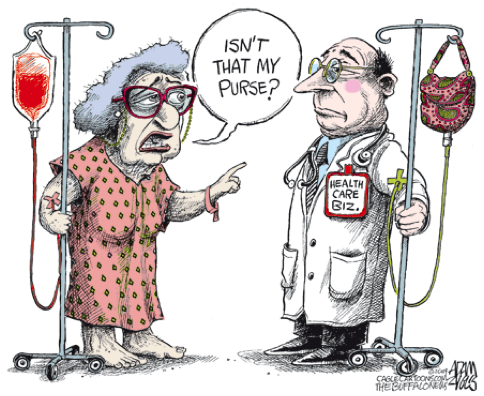
\includegraphics[scale=0.7]{Images/im17.png}
\end{center}
\end{figure}

\chapter{\'Etude de projets}

Les deux essais clinique ci-dessous ne sont pas terminés, c’est pourquoi il nous est impossible d’exploiter les résultats. 

Dans un premier temps nous étudierons un essai à l’échelle nationale : SHIVA, puis un deuxième à l’échelle internationale : WINTHER.

\section{SHIVA}

\subsection{Présentation de l’essai SHIVA}

L’institut Curie lance en octobre 2012 le projet SHIVA qui devrait durer trois ans. 

 \begin{figure}[H]
\begin{center}
    
\includegraphics[scale=1]{Images/im18.png}
\end{center}
\end{figure}

L’institut Curie est fondé en 1909 à Paris, sur un modèle conçu par Marie Curie. 
Cette dernière, née en 1867, est la seule femme à avoir reçu deux prix Nobel. Elle a été récompensée premièrement avec son mari Pierre Curie, par une moitié du prix Nobel de physique en 1903, pour leurs recherches sur les radiations, puis par le prix Nobel de chimie en 1911 pour ses travaux sur le polonium et le radium. 

L’institut est constitué à la fois d’un ensemble hospitalier et d’un centre de recherche. Son ensemble hospitalier rassemble 2000 personnes et représente une référence pour les cancers du sein, les tumeurs de l’œil et les cancers pédiatriques, sans oublier la prise en charge d’autres pathologies. Son centre de recherche est le centre dédié à la cancérologie le plus important de France et un des plus importants d’Europe. Il regroupe 1000 personnes de disciplines différentes, comme des biologistes, des physiciens, des chimistes ou des bio-informaticiens. L’institut Curie possède également un département de recherche translationnelle, depuis 2003, qui accélère le processus de passage de l’innovation scientifique à une meilleure prise en charge des patients.

Le coordinateur de ce projet est Christophe Le Tourneau, un oncologue médical de l’Institut Curie. Il dirige une équipe d’une dizaine de personnes au profils variés pour travailler sur cet essai clinique. Cet essai complexe et novateur est aussi multicentrique : plusieurs grands centres de recherches sont impliqués, comme à Paris, Lyon, Nantes, Marseille, Dijon, Nancy et Toulouse. C'est le premier essai clinique uniquement basé sur le profil biologique de la tumeur. En effet jusqu’à présent, les cancers étaient traités en fonction de la localisation de leur tumeur. Désormais, dans l’essai clinique SHIVA, grâce à des nouvelles techniques innovantes et moins coûteuses, il s’agirait de les soigner en fonction de la nature de leur tumeur. Pour cela, les chercheurs réalisent un prélèvement de la lésion cancéreuse et en établissent la carte génétique. Ensuite, les ingénieurs en bio-informatique repèrent les anomalies moléculaires et l’équipe médicale propose la thérapie ciblée correspondante.

Dans ce projet, environ 1000 patients en stade avancé de leur cancer et qui ne réagissent pas aux traitements existants seront testés. Le délai entre la première biopsie de la tumeur et la décision thérapeutique des bio-informaticiens devrait être entre 4 et 5 semaines pour chacun des patients.

\subsection{Les différentes étapes} 

 \begin{figure}[H]
\begin{center}
    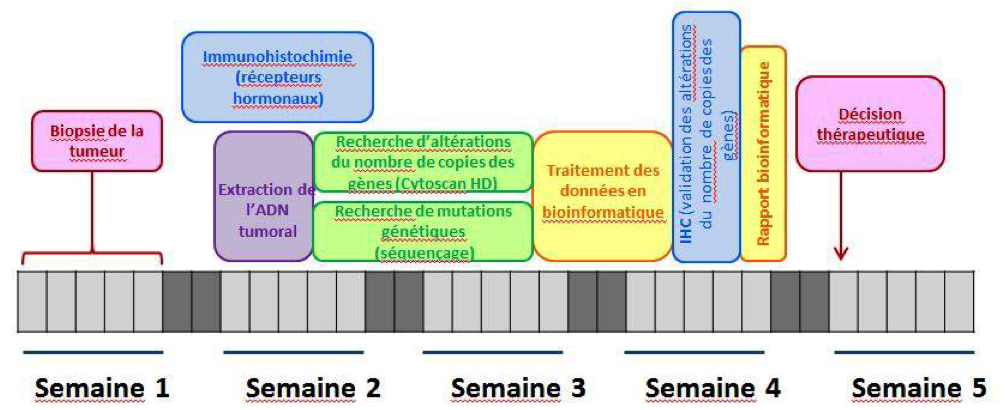
\includegraphics[scale=1]{Images/im19.png}
\caption{\'Etapes du protocole du projet SHIVA}    
\end{center}
\end{figure}

Premièrement, les patients subissent une biopsie. Le prélèvement est ensuite conservé dans des congélateurs à -80°C avant d’être étudié par les biologistes. Ainsi, ils peuvent confirmer s'il s’agit bien de tissus cancéreux ou non. Après confirmation, ils reprennent le reste du fragment de tumeur et le place dans une machine afin de le désintégrer. 

L'étape suivante consiste à extraire l'ADN\footnote{voir lexique page~\pageref{lexique}} grâce à une centrifugeuse. Pour examiner cet échantillon, les biologistes utilisent le séquençage, c’est à dire la détermination de la succession des nucléotides (Adénine, Thymine, Cytosine et Guanine) pour un fragment d’ADN donné : le brin matrice. Le séquençage fonctionne ainsi : \textit{une ADN polymérase (enzyme) synthétise le brin complémentaire de l’ADN à séquencer. Pour se faire, l’ADN polymérase utilise les nucléotides présents dans le milieu pour copier le brin matrice en synthétisant une ADN de séquence complémentaire, de sorte à toujours positionner un A en face d’un T, et un C en face d’un G. Cependant, dans le milieu, on trouve aussi une faible proportion d’un ddNTP (didésoxyribonucléotide), et quand celui-ci est ajouté par hasard à la chaîne en cours de synthèse par l’ADN polymérase, la synthèse du brin d’ADN s’arrête}. Les ingénieurs biologistes obtiennent ainsi la carte d’identité de l’ADN tumoral. Ils cherchent ensuite à comparer celle des personnes atteintes du cancer avec celle des personnes en bonne santé.

 \begin{figure}[H]
\begin{center}
    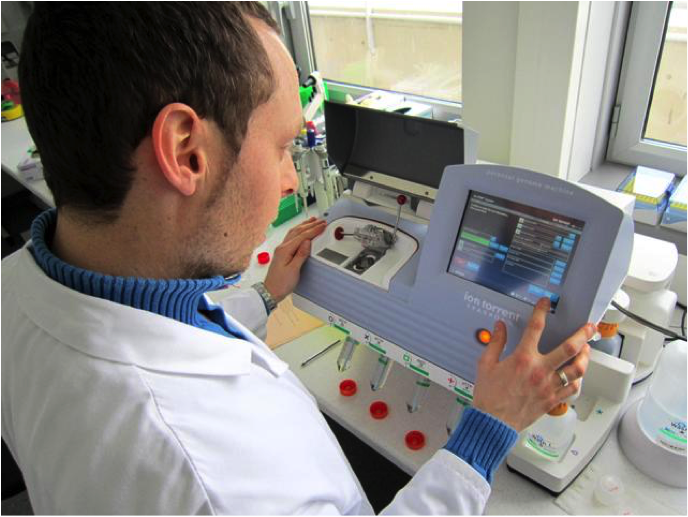
\includegraphics[scale=1]{Images/im20.png}
\caption{Séquençage à haut débit à l’Institut Curie}    
\end{center}
\end{figure}

Après une analyse biologique de chaque tumeur, les chercheurs peuvent déterminer si des anomalies sont présentes ou non dans la tumeur. Les patients présentant une anomalie moléculaire (mutations, amplifications de gènes, surexpression de récepteurs hormonaux\ldots) pour laquelle on possède une thérapie ciblée (environ 20\% attendus, selon Christophe Le Tourneau) seront répartis en deux groupes. L’un bénéficiera d’un traitement par chimiothérapie, et l’autre recevra une molécule ciblant l’anomalie moléculaire identifiée.

 \begin{figure}[H]
\begin{center}
    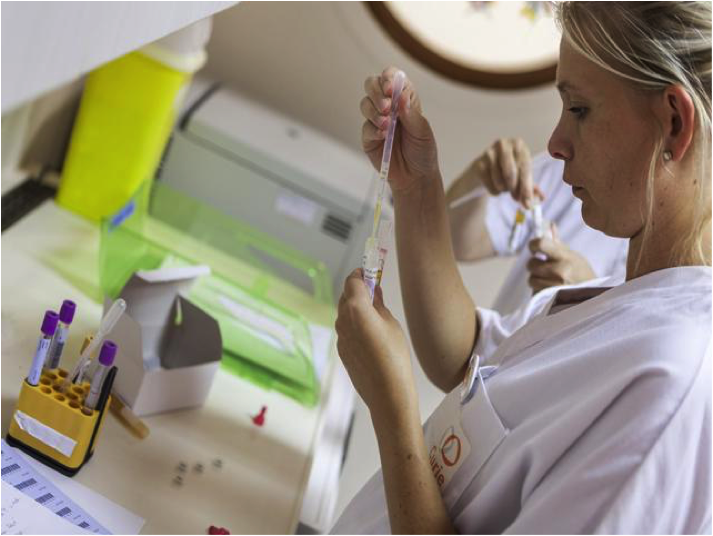
\includegraphics[scale=0.8]{Images/im21.png}
\caption{Analyse biologique à l’Institut Curie}    
\end{center}
\end{figure}

Une chimiothérapie classique agit sur les cellules tumorales, mais également sur les cellules saines, ce qui engendre des effets secondaires comme la perte de cheveux ou les nausées. 

Les thérapies ciblées, quant à elles, reconnaissent les cellules tumorales. Elles augmentent donc considérablement la qualité de soin et de vie des patients atteints du cancer. 

L’identification des cellules tumorales est possible grâce à la recherche d’anomalies moléculaires dans les prélèvements effectués sur le patient. Si, aujourd’hui, il n’existe sur le marché que 17 thérapies ciblées, plusieurs centaines sont en cours de développement à l’Institut Curie et dans les laboratoires, à échelle internationale. Grâce à elles, le cancer peut devenir une maladie chronique et non incurable.

\subsection{Bilan}

Le bilan actuel montre que, sur les cents premiers patients recrutés, la biopsie a pu être effectuée avec succès chez 95\% d’entre eux. Concernant la recherche de mutations, d’amplifications de gènes, et le dosage des récepteurs hormonaux, un résultat a pu être obtenu dans respectivement 66\%, 68\% et 92\% des cas. Au final, une thérapie ciblée a pu être administré dans 38\% des cas et le délai entre la biopsie et la décision thérapeutique a été de 26 jours en moyenne, soit moins de quatre semaines.

Ces résultats montrent que l’analyse du profil moléculaire de chaque tumeur est envisageable en routine dans des délais acceptables. 

Reste à savoir si cette stratégie est bénéfique pour les patients par rapport au schéma thérapeutique classique. "Nous regarderons si les traitements administrés en fonction de l’anomalie moléculaire font mieux que les traitements de référence par chimiothérapie pour stopper l’évolution des cancers", explique le docteur Christophe Le Tourneau. Pour cela, les chercheurs vont inclure toutes les localisations de cancers (sein, colon, pancréas…), sachant qu’aucune ne pourra représenter plus de 20\% des cas de la cohorte. « Pour valider ce concept de médecine personnalisée, il faut le vérifier sur une grande hétérogénéité de tumeurs", clarifie-t-il.

Environ 700 patients ont déjà été recrutés dans sept centres français de lutte contre le cancer  et les résultats d’efficacité sont attendus pour 2016. D’ici là, "il faudrait réfléchir à des moyens de ramener la période d’analyse de quatre à deux semaines, pour permettre une plus grande réactivité vis-à-vis des patients, notamment pour ceux dont les cancers évoluent rapidement", conclut le chercheur.

	Pour conclure, nous avons communiqué par le biais d’un mail, avec le coordinateur du projet SHIVA, Christophe Le Tourneau, car nous espérions obtenir des informations supplémentaires. Voici ce qu’il nous a répondu :

 \begin{figure}[H]
\begin{center}
    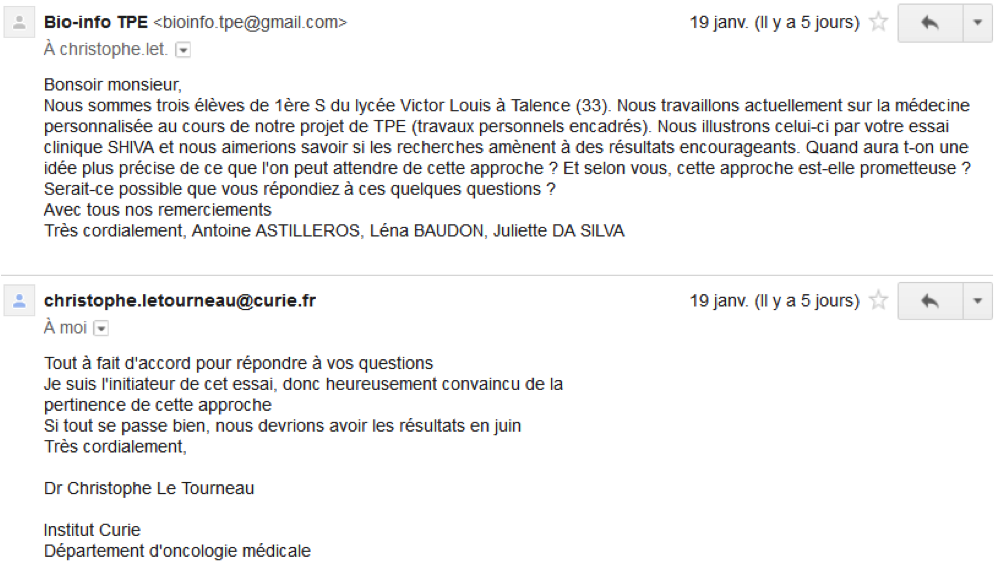
\includegraphics[scale=0.9]{Images/im22.png}
\end{center}
\end{figure}

\section{WINTHER}

\subsection{Présentation de l’essai WINTHER}

WINTHER est un essai clinique international globalement coordonné par le professeur cancérologue Jean-Charles Soria de l’institut Gustave-Roussy. 

 \begin{figure}[H]
\begin{center}
    
\includegraphics[scale=1]{Images/im23.png}
\end{center}
\end{figure}

L’Institut Gustave-Roussy, maintenant appelé Gustave-Roussy, est un centre régional de lutte contre le cancer situé à Villejuif dans le Val-de-Marne en France. Il fut créé en 1926 par Gustave Roussy, un neurologue, neuropathologiste et cancérologue d'origine Suisse, né en 1874. C’est le premier centre de soins, de recherche et d'enseignement en cancérologie d’Europe, avec ses quelques 2500 employés (chercheurs, médecins statutaires, personnels soignants…).

 L’essai WINTHER, qui a débuté en 2013, et dont les premiers résultats seraient attendus pour l’année 2015, est mené dans quatre pays : 
\begin{itemize}
\item en France, à Villejuif (Institut Gustave Roussy)
\item aux États-Unis, à Houston au Texas (M.D. Anderson Cancer Center)
\item en Espagne (Vall d’Hebron Hospital)
\item en Israël (The Chaim Sheba Medical Center)
\end{itemize}

\begin{figure}[htbp]
  \centering
  \subfloat[MD Anderson Cancer Center] {
    \centering

\includegraphics[width=5cm]{Images/im24.png}
}\hfill
\subfloat[Vall d’Hebron Hospital] { 
    \centering

\includegraphics[width=5cm]{Images/im25.png}
}\hfill
  \subfloat[The Chaim Sheba
  Medical Center] {
    \centering

\includegraphics[width =3cm]{Images/im26.png}
}
\end{figure}

Il vise à proposer un traitement personnalisé à une très grande majorité des patients, car jusqu’à présent, seulement un tiers des patients bénéficient d’un traitement personnalisé. L'essai se propose de comparer "la survie sans progression de la maladie" à l’aide de traitements guidés par l'analyse bio-informatique, à la survie avec des traitements standards.
L’essai compterait 200 patients atteints de différentes tumeurs solides métastatiques, ayant résistés à leur dernier traitement. Avec ce petit nombre de patients et comme l’essai ne devrait durer que deux ans, les scientifiques pourraient obtenir des résultats exploitables à court terme.
 
\subsection{Étapes de l’essai et bilan potentiel}

Dans un premier temps, une double biopsie de la tumeur (ou métastase) et du tissu sain de chaque patient devrait être réalisée. Ensuite, les ingénieurs réaliseraient une analyse biologique complète des ADN et  ARN à l’aide des techniques les plus modernes. Enfin, à partir de ces résultats, une liste de traitements serait proposée, avec un score prédictif d’efficacité pour les différentes thérapies. 

Pour 30\% des patients, le choix thérapeutique serait établi en fonction de ces analyses, car ils présentent une anomalie connue de l’ADN tumoral. Dans ce cas, une thérapie ciblée est donc disponible. 

Les 70\% des patients ne présentant pas d’anomalie connue de l’ADN tumoral auraient, eux, un choix thérapeutique orienté par les analyses de l’ARN tumoral et du tissu sain. Les résultats des analyses ADN, ARN et microARN\footnote{voir lexique page~\pageref{lexique}} de la tumeur et du tissu sain seront soumis à un programme bio-informatique capable de déterminer un score prédictif d’efficacité pour les différentes thérapies. La seule limite à l’approche est le succès du geste biopsique sur la tumeur et le tissu sain.

Ce système de score permet de prédire la réponse aux traitements existants sur le marché (standards ou ciblés, coûteux ou non) pour un patient donné. Cet outil bio-informatique complexe intègre toutes les données connues sur les biomarqueurs\footnote{voir lexique page~\pageref{lexique}}, les anomalies moléculaires et les thérapies ciblées ou non, et des algorithmes prédictifs d’efficacité.


\chapter{Conclusion}

La bio-informatique permet aux chercheurs de trouver les caractéristiques génétiques de la tumeur grâce aux séquençage d’ADN et à des algorithmes comme BLAST, afin de trouver un traitement compatible aux patients. Mais l’hétérogénéité intratumoral et le coût sont des problèmes dans le traitement des cancers grâce à la médecine personnalisé. 

Nous ne pouvons pas répondre à notre problématique qui était “la bio-informatique permet-elle vraiment d'aider au traitement des cancers ?” au jour d’aujourd’hui mais les essais SHIVA et WINTHER le permettront peut être. Nous avons rencontré Marie Beurton-Aimar\cite{BA2015}, une bio-informaticienne du Laboratoire Bordelais de Recherche en Informatique, qui a eu l’amabilité de répondre à nos questions et de nous éclaircir sur le sujet.    

\chapter*{Lexique}\label{lexique}

\begin{itemize}

\item Acide nucléique : terme désignant une substance constituée d’un enchaînement linéaire de nucléotides. Il en existe deux grandes catégories à l’état naturel : 
\begin{itemize}
\item ADN (Acide désoxyribonucléique) : l’ADN est une molécule très longue, composée d’une succession de nucléotides (A, T, C, G) accrochés les uns aux autres par des liaisons phosphodiester ;
\item ARN (Acide ribonucléique) : l’ARN est une molécule formée par l'enchaînement de quatre sortes de nucléotides (A, U, C, G), associés en un brin unique ;
\end{itemize}

\item Biomarqueur : un biomarqueur est une caractéristique mesurable qui représente un indicateur des processus biologiques normaux ou pathologiques ou un indicateur de réponse pharmacologique à une intervention thérapeutique.

\item Cancer métastatique : un cancer qui s'est propagé de son lieu d'origine (tumeur primitive) à une nouvelle partie du corps.

\item Génome : le génome est l’ensemble du matériel génétique d’un organisme.

\item Génotypage : il permet de connaître les variations génétiques (variants, allèles, nucléotides\ldots) d’une partie ou d’un génome entier.

\item MicroARN : les microARN ou “miRNA” en anglais, sont de courts acides ribonucléiques (ARN), simple-brins propres aux cellules eucaryotes. Ils possèdent en moyenne 22 nucléotides (en général de 21 à 24), soit beaucoup moins que les autres ARN.

\item Nucléotide : molécule constituée de l'enchaînement d’un groupement phosphate, d’un sucre et d’une base azotée.

\item Oncogène : qui favorise ou provoque le développement des tumeurs, notamment des tumeurs malignes.

\item Séquençage : détermine l’ordre d’enchaînement des nucluéotides pour un fragment d’ADN donné.

\item Métastase : une métastase est la croissance d'un organisme pathogène ou d'une cellule tumorale à distance du site initialement atteint par voie sanguine ou lymphatique.

\end{itemize}

\nocite{Andre2014, BA2015}

\bibliographystyle{unsrt}
\bibliography{bibliographie}


\end{document}

